\subsection{SERVIDOR E BANCO DE DADOS}

A aplicação do lado do servidor é responsável por receber as requisições da interface, persistir as configurações no banco de dados e realizar a comunicação com o otimizador, a fim de produzir e armazenar as grades horárias.

Para o desenvolvimento deste componente, optou-se pelo \textit{framework Express.js}, a ser executado na plataforma \textit{Node.js}, devido à simplicidade de implementação que estas tecnologias proporcionam. Em relação ao banco de dados, será utilizado o sistema de gerenciamento de banco de dados \textit{PostgresSQL}, devido à sua robustez e grande uso no mercado.

Conforme as premissas do problema sendo tratado, a modelagem do banco de dados visível na \autoref{fig:diagramaEr} é centrada na entidade ``Configuração'', que agrupa as configurações de determinada instituição de ensino para a geração de suas grades horárias. Cada uma dessas entidades tem turnos, turmas, professores, e as configurações de quantas aulas cada professor deve ministrar para cada turma, e as respectivas restrições.

\begin{figure}[!htb]
	\centering
	\caption{Modelo Entidade-Relacionamento}
	\includegraphics[width=1\textwidth]{./dados/figuras/ER_horario_INCREMENTO3}
	\fonte{Autor}
	\label{fig:diagramaEr}
\end{figure}
\newpage

Na \autoref{fig:diagramaEr}, é possível notar a presença das entidades elacionadas às diversas métricas de qualidade comentadas na \autoref{subsec:pesos_e_restricoes}, como restrições, contrantes, regiões, grupos de alinhamento, entre outras.

As figuras \ref{fig:sqlValidacao} e \ref{fig:consultaGrade} demonstram algumas inserções e resultados de consultas utilizadas para validar a modelagem.

\begin{figure}[h]
	\centering
	\caption{Consultas de validação da modelagem}
	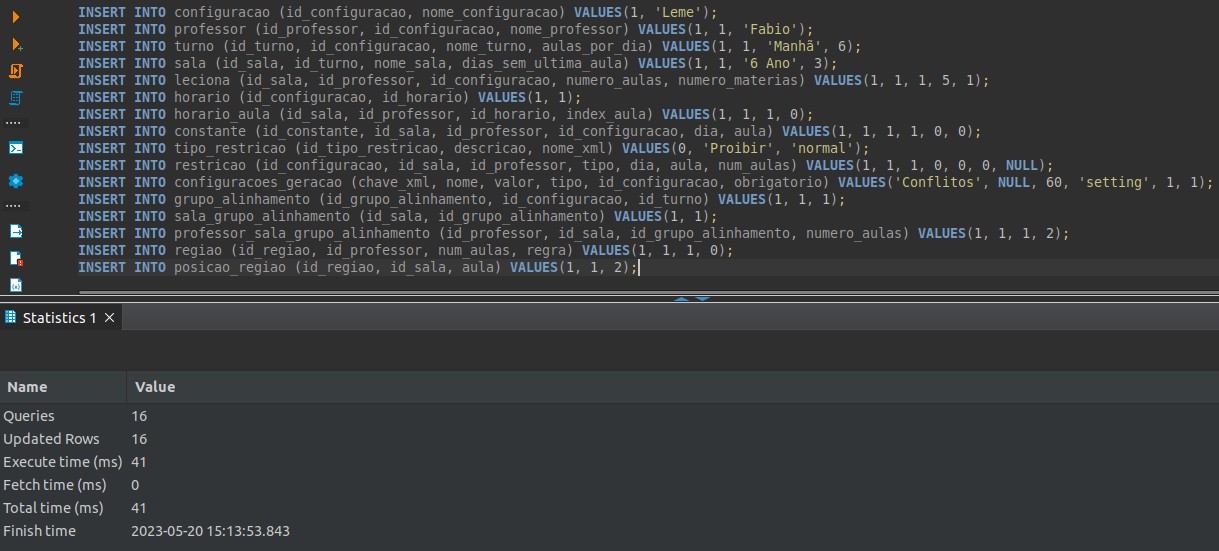
\includegraphics[width=1\textwidth]{./dados/figuras/sql_validacao}
	\fonte{Autor}
	\label{fig:sqlValidacao}
\end{figure}

\begin{figure}[h]
	\centering
	\caption{Resultado da consulta de uma grade no banco de dados}
	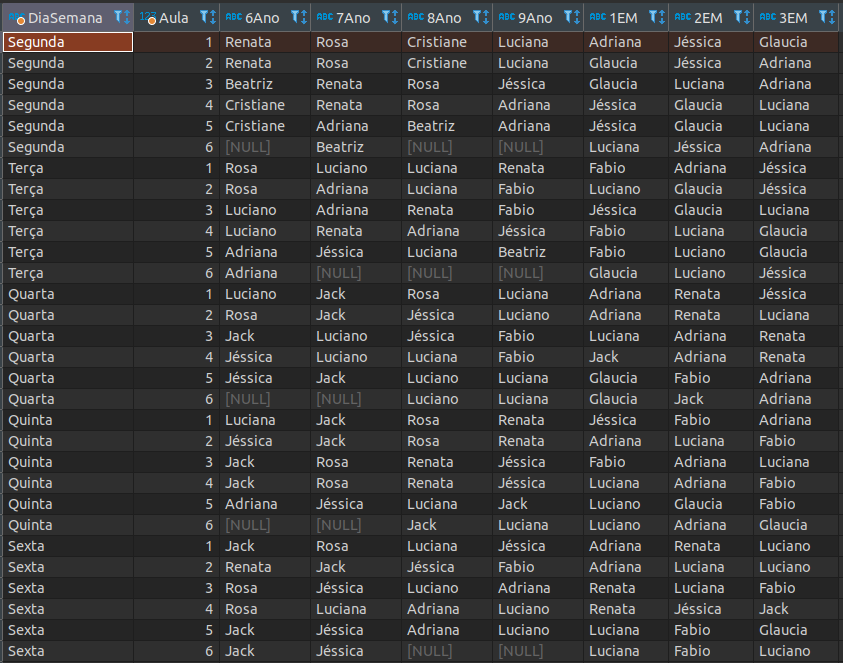
\includegraphics[width=0.7\textwidth]{./dados/figuras/ConsultaGrade}
	\fonte{Autor}
	\label{fig:consultaGrade}
\end{figure}